\documentclass[twoside]{book}

% Packages required by doxygen
\usepackage{fixltx2e}
\usepackage{calc}
\usepackage{doxygen}
\usepackage[export]{adjustbox} % also loads graphicx
\usepackage{graphicx}
\usepackage[utf8]{inputenc}
\usepackage{makeidx}
\usepackage{multicol}
\usepackage{multirow}
\PassOptionsToPackage{warn}{textcomp}
\usepackage{textcomp}
\usepackage[nointegrals]{wasysym}
\usepackage[table]{xcolor}

% NLS support packages
\usepackage[brazil]{babel}
% Font selection
\usepackage[T1]{fontenc}
\usepackage[scaled=.90]{helvet}
\usepackage{courier}
\usepackage{amssymb}
\usepackage{sectsty}
\renewcommand{\familydefault}{\sfdefault}
\allsectionsfont{%
  \fontseries{bc}\selectfont%
  \color{darkgray}%
}
\renewcommand{\DoxyLabelFont}{%
  \fontseries{bc}\selectfont%
  \color{darkgray}%
}
\newcommand{\+}{\discretionary{\mbox{\scriptsize$\hookleftarrow$}}{}{}}

% Page & text layout
\usepackage{geometry}
\geometry{%
  a4paper,%
  top=2.5cm,%
  bottom=2.5cm,%
  left=2.5cm,%
  right=2.5cm%
}
\tolerance=750
\hfuzz=15pt
\hbadness=750
\setlength{\emergencystretch}{15pt}
\setlength{\parindent}{0cm}
\setlength{\parskip}{3ex plus 2ex minus 2ex}
\makeatletter
\renewcommand{\paragraph}{%
  \@startsection{paragraph}{4}{0ex}{-1.0ex}{1.0ex}{%
    \normalfont\normalsize\bfseries\SS@parafont%
  }%
}
\renewcommand{\subparagraph}{%
  \@startsection{subparagraph}{5}{0ex}{-1.0ex}{1.0ex}{%
    \normalfont\normalsize\bfseries\SS@subparafont%
  }%
}
\makeatother

% Headers & footers
\usepackage{fancyhdr}
\pagestyle{fancyplain}
\fancyhead[LE]{\fancyplain{}{\bfseries\thepage}}
\fancyhead[CE]{\fancyplain{}{}}
\fancyhead[RE]{\fancyplain{}{\bfseries\leftmark}}
\fancyhead[LO]{\fancyplain{}{\bfseries\rightmark}}
\fancyhead[CO]{\fancyplain{}{}}
\fancyhead[RO]{\fancyplain{}{\bfseries\thepage}}
\fancyfoot[LE]{\fancyplain{}{}}
\fancyfoot[CE]{\fancyplain{}{}}
\fancyfoot[RE]{\fancyplain{}{\bfseries\scriptsize Gerado por Doxygen }}
\fancyfoot[LO]{\fancyplain{}{\bfseries\scriptsize Gerado por Doxygen }}
\fancyfoot[CO]{\fancyplain{}{}}
\fancyfoot[RO]{\fancyplain{}{}}
\renewcommand{\footrulewidth}{0.4pt}
\renewcommand{\chaptermark}[1]{%
  \markboth{#1}{}%
}
\renewcommand{\sectionmark}[1]{%
  \markright{\thesection\ #1}%
}

% Indices & bibliography
\usepackage{natbib}
\usepackage[titles]{tocloft}
\setcounter{tocdepth}{3}
\setcounter{secnumdepth}{5}
\makeindex

% Hyperlinks (required, but should be loaded last)
\usepackage{ifpdf}
\ifpdf
  \usepackage[pdftex,pagebackref=true]{hyperref}
\else
  \usepackage[ps2pdf,pagebackref=true]{hyperref}
\fi
\hypersetup{%
  colorlinks=true,%
  linkcolor=blue,%
  citecolor=blue,%
  unicode%
}

% Custom commands
\newcommand{\clearemptydoublepage}{%
  \newpage{\pagestyle{empty}\cleardoublepage}%
}

\usepackage{caption}
\captionsetup{labelsep=space,justification=centering,font={bf},singlelinecheck=off,skip=4pt,position=top}

%===== C O N T E N T S =====

\begin{document}

% Titlepage & ToC
\hypersetup{pageanchor=false,
             bookmarksnumbered=true,
             pdfencoding=unicode
            }
\pagenumbering{alph}
\begin{titlepage}
\vspace*{7cm}
\begin{center}%
{\Large Classe Abstrata \\[1ex]\large O\+MG }\\
\vspace*{1cm}
{\large Gerado por Doxygen 1.8.14}\\
\end{center}
\end{titlepage}
\clearemptydoublepage
\pagenumbering{roman}
\tableofcontents
\clearemptydoublepage
\pagenumbering{arabic}
\hypersetup{pageanchor=true}

%--- Begin generated contents ---
\chapter{Índice Hierárquico}
\section{Hierarquia de Classes}
Esta lista de hierarquias está parcialmente ordenada (ordem alfabética)\+:\begin{DoxyCompactList}
\item \contentsline{section}{Classes\+\_\+\+Abstratas}{\pageref{class_classes___abstratas}}{}
\item \contentsline{section}{Figura\+Geometrica}{\pageref{class_figura_geometrica}}{}
\begin{DoxyCompactList}
\item \contentsline{section}{Circulo}{\pageref{class_circulo}}{}
\item \contentsline{section}{Ponto}{\pageref{class_ponto}}{}
\item \contentsline{section}{Reta}{\pageref{class_reta}}{}
\item \contentsline{section}{Retangulo}{\pageref{class_retangulo}}{}
\end{DoxyCompactList}
\item \contentsline{section}{Screen}{\pageref{class_screen}}{}
\end{DoxyCompactList}

\chapter{Índice dos Componentes}
\section{Lista de Classes}
Aqui estão as classes, estruturas, uniões e interfaces e suas respectivas descrições\+:\begin{DoxyCompactList}
\item\contentsline{section}{\mbox{\hyperlink{class_circulo}{Circulo}} \\*A classe \mbox{\hyperlink{class_circulo}{Circulo}} serve para construir a base do círculo }{\pageref{class_circulo}}{}
\item\contentsline{section}{\mbox{\hyperlink{class_classes___abstratas}{Classes\+\_\+\+Abstratas}} }{\pageref{class_classes___abstratas}}{}
\item\contentsline{section}{\mbox{\hyperlink{class_figura_geometrica}{Figura\+Geometrica}} \\*A classe \mbox{\hyperlink{class_figura_geometrica}{Figura\+Geometrica}} é a classe origem do projeto }{\pageref{class_figura_geometrica}}{}
\item\contentsline{section}{\mbox{\hyperlink{class_ponto}{Ponto}} }{\pageref{class_ponto}}{}
\item\contentsline{section}{\mbox{\hyperlink{class_reta}{Reta}} \\*A classe \mbox{\hyperlink{class_reta}{Reta}} serve para construir a base da reta }{\pageref{class_reta}}{}
\item\contentsline{section}{\mbox{\hyperlink{class_retangulo}{Retangulo}} \\*A classe \mbox{\hyperlink{class_retangulo}{Retangulo}} serve para construir a base do retângulo }{\pageref{class_retangulo}}{}
\item\contentsline{section}{\mbox{\hyperlink{class_screen}{Screen}} \\*A classe \mbox{\hyperlink{class_screen}{Screen}} construção da tela e toda base de informações para constuir os desenhos }{\pageref{class_screen}}{}
\end{DoxyCompactList}

\chapter{Classes}
\hypertarget{class_circulo}{}\section{Referência da Classe Circulo}
\label{class_circulo}\index{Circulo@{Circulo}}


A classe \mbox{\hyperlink{class_circulo}{Circulo}} serve para construir a base do círculo.  




{\ttfamily \#include $<$circulo.\+h$>$}

Diagrama de hierarquia para Circulo\+:\begin{figure}[H]
\begin{center}
\leavevmode
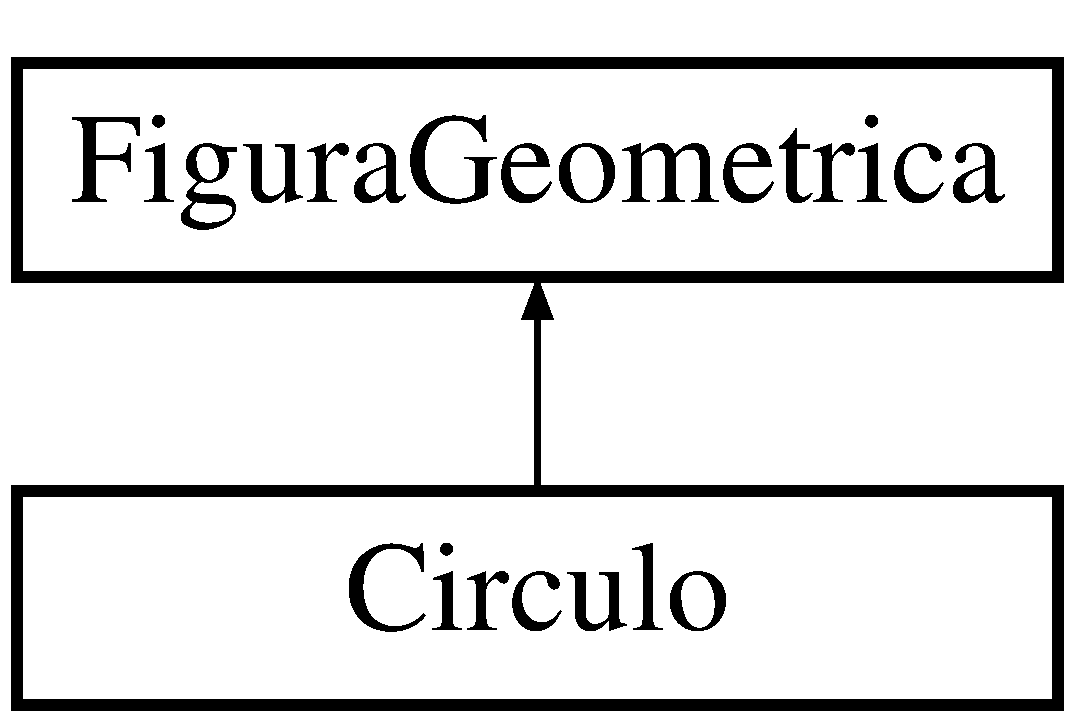
\includegraphics[height=2.000000cm]{class_circulo}
\end{center}
\end{figure}
\subsection*{Membros Públicos}
\begin{DoxyCompactItemize}
\item 
\mbox{\hyperlink{class_circulo_adbd3016265651b29c514d52f2b31adef}{Circulo}} (int x\+\_\+, int y\+\_\+, int raio\+\_\+, bool fill\+\_\+)
\begin{DoxyCompactList}\small\item\em \mbox{\hyperlink{class_circulo}{Circulo}} é o método construtor da classe \mbox{\hyperlink{class_circulo}{Circulo}}. \end{DoxyCompactList}\item 
void \mbox{\hyperlink{class_circulo_a593787d6e0618c2eded23e8839e7bea6}{draw}} (\mbox{\hyperlink{class_screen}{Screen}} \&t)
\begin{DoxyCompactList}\small\item\em draw é o método da classe \mbox{\hyperlink{class_figura_geometrica}{Figura\+Geometrica}} que serve para desenhar o círculo. \end{DoxyCompactList}\end{DoxyCompactItemize}


\subsection{Descrição detalhada}
A classe \mbox{\hyperlink{class_circulo}{Circulo}} serve para construir a base do círculo. 

\subsection{Construtores e Destrutores}
\mbox{\Hypertarget{class_circulo_adbd3016265651b29c514d52f2b31adef}\label{class_circulo_adbd3016265651b29c514d52f2b31adef}} 
\index{Circulo@{Circulo}!Circulo@{Circulo}}
\index{Circulo@{Circulo}!Circulo@{Circulo}}
\subsubsection{\texorpdfstring{Circulo()}{Circulo()}}
{\footnotesize\ttfamily Circulo\+::\+Circulo (\begin{DoxyParamCaption}\item[{int}]{x\+\_\+,  }\item[{int}]{y\+\_\+,  }\item[{int}]{raio\+\_\+,  }\item[{bool}]{fill\+\_\+ }\end{DoxyParamCaption})}



\mbox{\hyperlink{class_circulo}{Circulo}} é o método construtor da classe \mbox{\hyperlink{class_circulo}{Circulo}}. 


\begin{DoxyParams}{Parâmetros}
{\em x\+\_\+} & é a coordenada X do ponto no centro do círculo.\\
\hline
{\em y\+\_\+} & é a coordenada Y do ponto no centro do círculo.\\
\hline
{\em raio\+\_\+} & é o valor do raio do círculo.\\
\hline
{\em fill\+\_\+} & é o tipo do preenchimento. 1 -\/ cheio e 0 -\/ vazio \\
\hline
\end{DoxyParams}


\subsection{Funções membros}
\mbox{\Hypertarget{class_circulo_a593787d6e0618c2eded23e8839e7bea6}\label{class_circulo_a593787d6e0618c2eded23e8839e7bea6}} 
\index{Circulo@{Circulo}!draw@{draw}}
\index{draw@{draw}!Circulo@{Circulo}}
\subsubsection{\texorpdfstring{draw()}{draw()}}
{\footnotesize\ttfamily void Circulo\+::draw (\begin{DoxyParamCaption}\item[{\mbox{\hyperlink{class_screen}{Screen}} \&}]{t }\end{DoxyParamCaption})\hspace{0.3cm}{\ttfamily [virtual]}}



draw é o método da classe \mbox{\hyperlink{class_figura_geometrica}{Figura\+Geometrica}} que serve para desenhar o círculo. 


\begin{DoxyParams}{Parâmetros}
{\em t} & é um ponteiro para uma variável do tipo \mbox{\hyperlink{class_screen}{Screen}} (variável da tela) . \\
\hline
\end{DoxyParams}


Implementa \mbox{\hyperlink{class_figura_geometrica_a8ee8dedc060b6059a805ea091aef2c41}{Figura\+Geometrica}}.



A documentação para essa classe foi gerada a partir dos seguintes arquivos\+:\begin{DoxyCompactItemize}
\item 
circulo.\+h\item 
circulo.\+cpp\end{DoxyCompactItemize}

\hypertarget{class_classes___abstratas}{}\section{Referência da Classe Classes\+\_\+\+Abstratas}
\label{class_classes___abstratas}\index{Classes\+\_\+\+Abstratas@{Classes\+\_\+\+Abstratas}}
\subsection*{Membros Públicos}
\begin{DoxyCompactItemize}
\item 
\mbox{\Hypertarget{class_classes___abstratas_a5d4807c842f739f07a61e8000dda0f48}\label{class_classes___abstratas_a5d4807c842f739f07a61e8000dda0f48}} 
\mbox{\hyperlink{class_classes___abstratas_a5d4807c842f739f07a61e8000dda0f48}{Classes\+\_\+\+Abstratas}} ()
\begin{DoxyCompactList}\small\item\em \mbox{\hyperlink{class_classes___abstratas}{Classes\+\_\+\+Abstratas}} é o construtor da classe \mbox{\hyperlink{class_classes___abstratas}{Classes\+\_\+\+Abstratas}}. \end{DoxyCompactList}\end{DoxyCompactItemize}


A documentação para essa classe foi gerada a partir dos seguintes arquivos\+:\begin{DoxyCompactItemize}
\item 
classes\+\_\+abstratas.\+h\item 
classes\+\_\+abstratas.\+cpp\end{DoxyCompactItemize}

\hypertarget{class_figura_geometrica}{}\section{Referência da Classe Figura\+Geometrica}
\label{class_figura_geometrica}\index{Figura\+Geometrica@{Figura\+Geometrica}}


A classe \mbox{\hyperlink{class_figura_geometrica}{Figura\+Geometrica}} é a classe origem do projeto.  




{\ttfamily \#include $<$figurageometrica.\+h$>$}

Diagrama de hierarquia para Figura\+Geometrica\+:\begin{figure}[H]
\begin{center}
\leavevmode
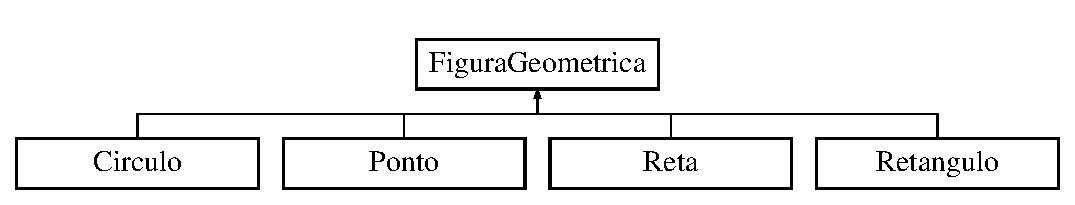
\includegraphics[height=2.000000cm]{class_figura_geometrica}
\end{center}
\end{figure}
\subsection*{Membros Públicos}
\begin{DoxyCompactItemize}
\item 
virtual void \mbox{\hyperlink{class_figura_geometrica_a8ee8dedc060b6059a805ea091aef2c41}{draw}} (\mbox{\hyperlink{class_screen}{Screen}} \&t)=0
\begin{DoxyCompactList}\small\item\em \mbox{\hyperlink{class_figura_geometrica}{Figura\+Geometrica}} é o construtor da classe \mbox{\hyperlink{class_figura_geometrica}{Figura\+Geometrica}}. \end{DoxyCompactList}\end{DoxyCompactItemize}


\subsection{Descrição detalhada}
A classe \mbox{\hyperlink{class_figura_geometrica}{Figura\+Geometrica}} é a classe origem do projeto. 

\subsection{Funções membros}
\mbox{\Hypertarget{class_figura_geometrica_a8ee8dedc060b6059a805ea091aef2c41}\label{class_figura_geometrica_a8ee8dedc060b6059a805ea091aef2c41}} 
\index{Figura\+Geometrica@{Figura\+Geometrica}!draw@{draw}}
\index{draw@{draw}!Figura\+Geometrica@{Figura\+Geometrica}}
\subsubsection{\texorpdfstring{draw()}{draw()}}
{\footnotesize\ttfamily virtual void Figura\+Geometrica\+::draw (\begin{DoxyParamCaption}\item[{\mbox{\hyperlink{class_screen}{Screen}} \&}]{t }\end{DoxyParamCaption})\hspace{0.3cm}{\ttfamily [pure virtual]}}



\mbox{\hyperlink{class_figura_geometrica}{Figura\+Geometrica}} é o construtor da classe \mbox{\hyperlink{class_figura_geometrica}{Figura\+Geometrica}}. 

draw é o método para desenhar usado em todas as classes herdeiras da \mbox{\hyperlink{class_figura_geometrica}{Figura\+Geometrica}}. Serve para desenhar as figuras geométricas. 
\begin{DoxyParams}{Parâmetros}
{\em t} & é um ponteiro para uma variável do tipo \mbox{\hyperlink{class_screen}{Screen}}. \\
\hline
\end{DoxyParams}


Implementado por \mbox{\hyperlink{class_circulo_a593787d6e0618c2eded23e8839e7bea6}{Circulo}}, \mbox{\hyperlink{class_retangulo_ac088dd6d3f4f3d3f80363a868c2e74f1}{Retangulo}}, \mbox{\hyperlink{class_reta_ac2e9805183cd474b62bffd8b032cd780}{Reta}} e \mbox{\hyperlink{class_ponto_acc49c2522288aea2819458f245bbc9df}{Ponto}}.



A documentação para essa classe foi gerada a partir do seguinte arquivo\+:\begin{DoxyCompactItemize}
\item 
figurageometrica.\+h\end{DoxyCompactItemize}

\hypertarget{class_ponto}{}\section{Referência da Classe Ponto}
\label{class_ponto}\index{Ponto@{Ponto}}
Diagrama de hierarquia para Ponto\+:\begin{figure}[H]
\begin{center}
\leavevmode
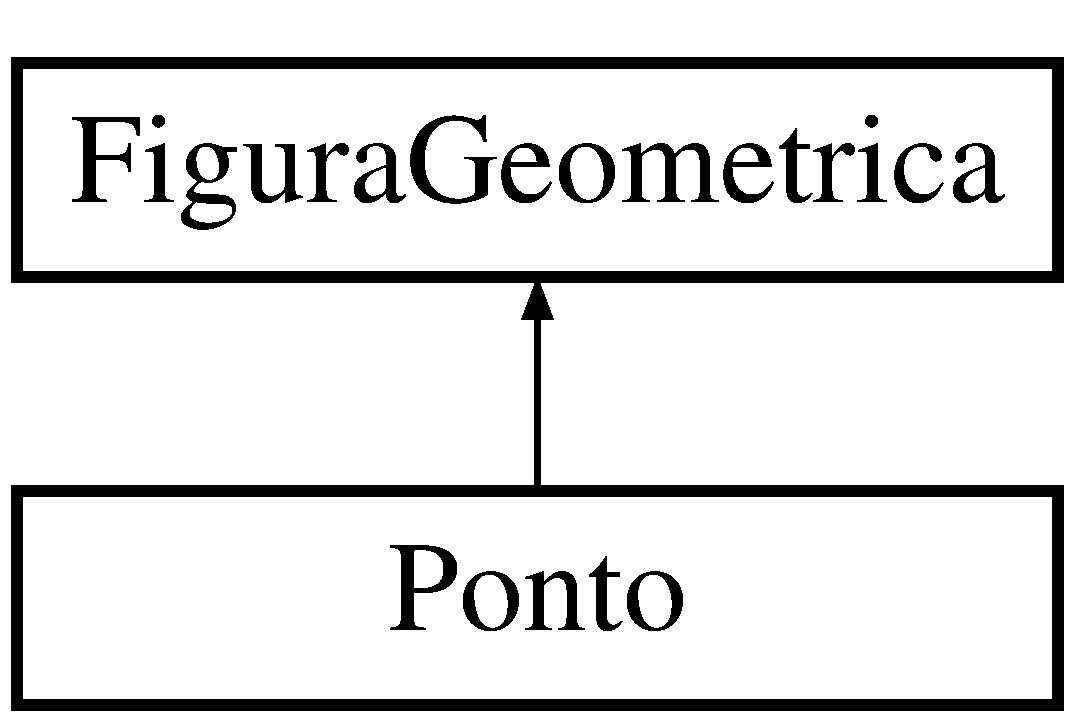
\includegraphics[height=2.000000cm]{class_ponto}
\end{center}
\end{figure}
\subsection*{Membros Públicos}
\begin{DoxyCompactItemize}
\item 
\mbox{\Hypertarget{class_ponto_a12ce1ad29a82da82ceb4c7d638bc46b9}\label{class_ponto_a12ce1ad29a82da82ceb4c7d638bc46b9}} 
{\bfseries Ponto} (int \+\_\+x, int \+\_\+y, char brush\+\_\+)
\item 
void \mbox{\hyperlink{class_ponto_acc49c2522288aea2819458f245bbc9df}{draw}} (\mbox{\hyperlink{class_screen}{Screen}} \&t)
\begin{DoxyCompactList}\small\item\em \mbox{\hyperlink{class_figura_geometrica}{Figura\+Geometrica}} é o construtor da classe \mbox{\hyperlink{class_figura_geometrica}{Figura\+Geometrica}}. \end{DoxyCompactList}\end{DoxyCompactItemize}


\subsection{Funções membros}
\mbox{\Hypertarget{class_ponto_acc49c2522288aea2819458f245bbc9df}\label{class_ponto_acc49c2522288aea2819458f245bbc9df}} 
\index{Ponto@{Ponto}!draw@{draw}}
\index{draw@{draw}!Ponto@{Ponto}}
\subsubsection{\texorpdfstring{draw()}{draw()}}
{\footnotesize\ttfamily void Ponto\+::draw (\begin{DoxyParamCaption}\item[{\mbox{\hyperlink{class_screen}{Screen}} \&}]{t }\end{DoxyParamCaption})\hspace{0.3cm}{\ttfamily [virtual]}}



\mbox{\hyperlink{class_figura_geometrica}{Figura\+Geometrica}} é o construtor da classe \mbox{\hyperlink{class_figura_geometrica}{Figura\+Geometrica}}. 

draw é o método para desenhar usado em todas as classes herdeiras da \mbox{\hyperlink{class_figura_geometrica}{Figura\+Geometrica}}. Serve para desenhar as figuras geométricas. 
\begin{DoxyParams}{Parâmetros}
{\em t} & é um ponteiro para uma variável do tipo \mbox{\hyperlink{class_screen}{Screen}}. \\
\hline
\end{DoxyParams}


Implementa \mbox{\hyperlink{class_figura_geometrica_a8ee8dedc060b6059a805ea091aef2c41}{Figura\+Geometrica}}.



A documentação para essa classe foi gerada a partir dos seguintes arquivos\+:\begin{DoxyCompactItemize}
\item 
ponto.\+h\item 
ponto.\+cpp\end{DoxyCompactItemize}

\hypertarget{class_reta}{}\section{Referência da Classe Reta}
\label{class_reta}\index{Reta@{Reta}}


A classe \mbox{\hyperlink{class_reta}{Reta}} serve para construir a base da reta.  




{\ttfamily \#include $<$reta.\+h$>$}

Diagrama de hierarquia para Reta\+:\begin{figure}[H]
\begin{center}
\leavevmode
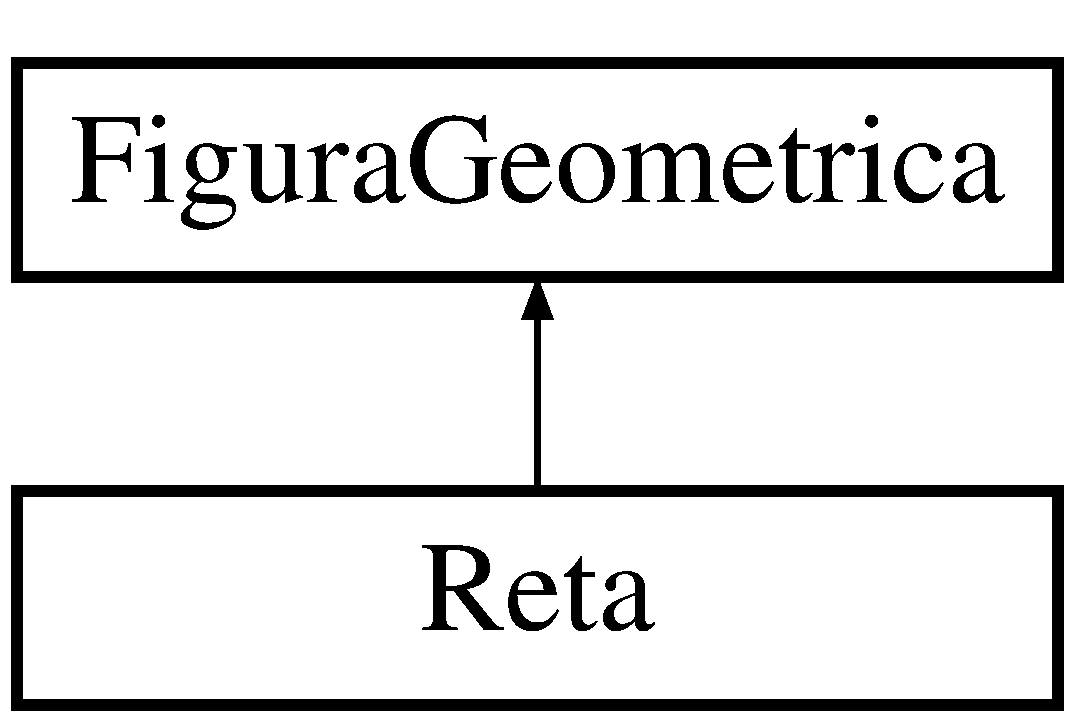
\includegraphics[height=2.000000cm]{class_reta}
\end{center}
\end{figure}
\subsection*{Membros Públicos}
\begin{DoxyCompactItemize}
\item 
\mbox{\Hypertarget{class_reta_a78ddb282fcaf38ff9cda2dc0f419cef2}\label{class_reta_a78ddb282fcaf38ff9cda2dc0f419cef2}} 
{\bfseries Reta} (int xa\+\_\+, int ya\+\_\+, int xb\+\_\+, int yb\+\_\+)
\item 
void \mbox{\hyperlink{class_reta_ac2e9805183cd474b62bffd8b032cd780}{draw}} (\mbox{\hyperlink{class_screen}{Screen}} \&t)
\begin{DoxyCompactList}\small\item\em \mbox{\hyperlink{class_figura_geometrica}{Figura\+Geometrica}} é o construtor da classe \mbox{\hyperlink{class_figura_geometrica}{Figura\+Geometrica}}. \end{DoxyCompactList}\end{DoxyCompactItemize}


\subsection{Descrição detalhada}
A classe \mbox{\hyperlink{class_reta}{Reta}} serve para construir a base da reta. 

\subsection{Funções membros}
\mbox{\Hypertarget{class_reta_ac2e9805183cd474b62bffd8b032cd780}\label{class_reta_ac2e9805183cd474b62bffd8b032cd780}} 
\index{Reta@{Reta}!draw@{draw}}
\index{draw@{draw}!Reta@{Reta}}
\subsubsection{\texorpdfstring{draw()}{draw()}}
{\footnotesize\ttfamily void Reta\+::draw (\begin{DoxyParamCaption}\item[{\mbox{\hyperlink{class_screen}{Screen}} \&}]{t }\end{DoxyParamCaption})\hspace{0.3cm}{\ttfamily [virtual]}}



\mbox{\hyperlink{class_figura_geometrica}{Figura\+Geometrica}} é o construtor da classe \mbox{\hyperlink{class_figura_geometrica}{Figura\+Geometrica}}. 

draw é o método para desenhar usado em todas as classes herdeiras da \mbox{\hyperlink{class_figura_geometrica}{Figura\+Geometrica}}. Serve para desenhar as figuras geométricas. 
\begin{DoxyParams}{Parâmetros}
{\em t} & é um ponteiro para uma variável do tipo \mbox{\hyperlink{class_screen}{Screen}}. \\
\hline
\end{DoxyParams}


Implementa \mbox{\hyperlink{class_figura_geometrica_a8ee8dedc060b6059a805ea091aef2c41}{Figura\+Geometrica}}.



A documentação para essa classe foi gerada a partir dos seguintes arquivos\+:\begin{DoxyCompactItemize}
\item 
reta.\+h\item 
reta.\+cpp\end{DoxyCompactItemize}

\hypertarget{class_retangulo}{}\section{Referência da Classe Retangulo}
\label{class_retangulo}\index{Retangulo@{Retangulo}}


A classe \mbox{\hyperlink{class_retangulo}{Retangulo}} serve para construir a base do retângulo.  




{\ttfamily \#include $<$retangulo.\+h$>$}

Diagrama de hierarquia para Retangulo\+:\begin{figure}[H]
\begin{center}
\leavevmode
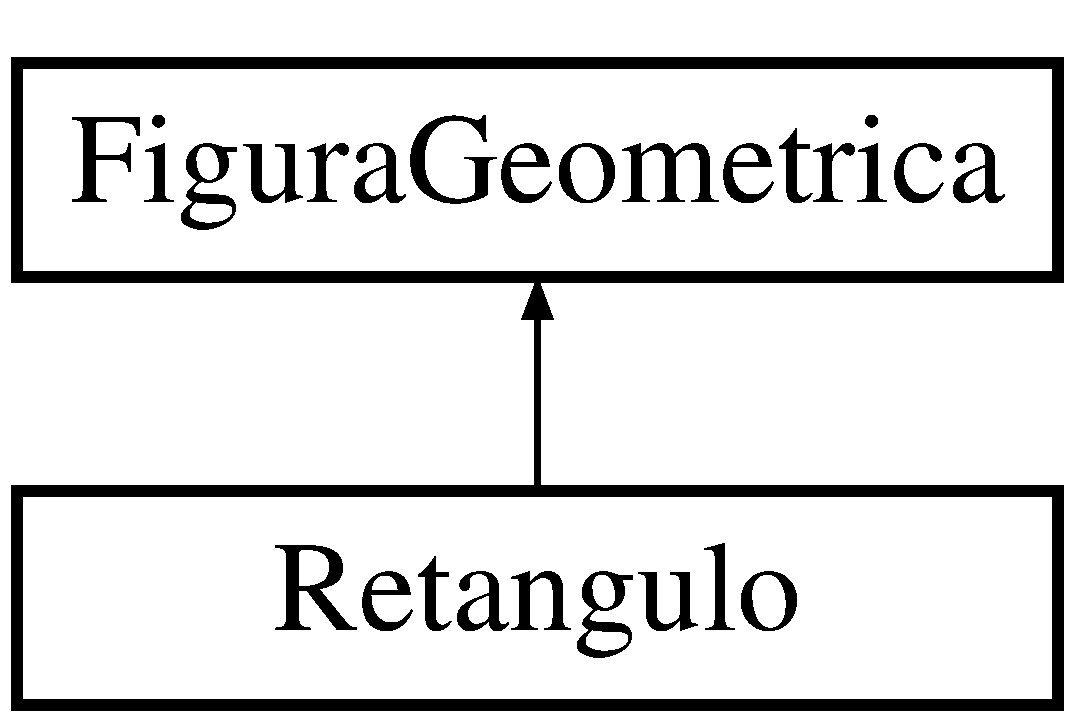
\includegraphics[height=2.000000cm]{class_retangulo}
\end{center}
\end{figure}
\subsection*{Membros Públicos}
\begin{DoxyCompactItemize}
\item 
\mbox{\Hypertarget{class_retangulo_aacd2438d0f0a119c5a9358c3da7c9eee}\label{class_retangulo_aacd2438d0f0a119c5a9358c3da7c9eee}} 
{\bfseries Retangulo} (int x\+\_\+, int y\+\_\+, int larg\+\_\+, int alt\+\_\+, bool fill\+\_\+)
\item 
void \mbox{\hyperlink{class_retangulo_ac088dd6d3f4f3d3f80363a868c2e74f1}{draw}} (\mbox{\hyperlink{class_screen}{Screen}} \&t)
\begin{DoxyCompactList}\small\item\em \mbox{\hyperlink{class_figura_geometrica}{Figura\+Geometrica}} é o construtor da classe \mbox{\hyperlink{class_figura_geometrica}{Figura\+Geometrica}}. \end{DoxyCompactList}\end{DoxyCompactItemize}


\subsection{Descrição detalhada}
A classe \mbox{\hyperlink{class_retangulo}{Retangulo}} serve para construir a base do retângulo. 

\subsection{Funções membros}
\mbox{\Hypertarget{class_retangulo_ac088dd6d3f4f3d3f80363a868c2e74f1}\label{class_retangulo_ac088dd6d3f4f3d3f80363a868c2e74f1}} 
\index{Retangulo@{Retangulo}!draw@{draw}}
\index{draw@{draw}!Retangulo@{Retangulo}}
\subsubsection{\texorpdfstring{draw()}{draw()}}
{\footnotesize\ttfamily void Retangulo\+::draw (\begin{DoxyParamCaption}\item[{\mbox{\hyperlink{class_screen}{Screen}} \&}]{t }\end{DoxyParamCaption})\hspace{0.3cm}{\ttfamily [virtual]}}



\mbox{\hyperlink{class_figura_geometrica}{Figura\+Geometrica}} é o construtor da classe \mbox{\hyperlink{class_figura_geometrica}{Figura\+Geometrica}}. 

draw é o método para desenhar usado em todas as classes herdeiras da \mbox{\hyperlink{class_figura_geometrica}{Figura\+Geometrica}}. Serve para desenhar as figuras geométricas. 
\begin{DoxyParams}{Parâmetros}
{\em t} & é um ponteiro para uma variável do tipo \mbox{\hyperlink{class_screen}{Screen}}. \\
\hline
\end{DoxyParams}


Implementa \mbox{\hyperlink{class_figura_geometrica_a8ee8dedc060b6059a805ea091aef2c41}{Figura\+Geometrica}}.



A documentação para essa classe foi gerada a partir dos seguintes arquivos\+:\begin{DoxyCompactItemize}
\item 
retangulo.\+h\item 
retangulo.\+cpp\end{DoxyCompactItemize}

\hypertarget{class_screen}{}\section{Referência da Classe Screen}
\label{class_screen}\index{Screen@{Screen}}


A classe \mbox{\hyperlink{class_screen}{Screen}} construção da tela e toda base de informações para constuir os desenhos.  




{\ttfamily \#include $<$screen.\+h$>$}

\subsection*{Membros Públicos}
\begin{DoxyCompactItemize}
\item 
\mbox{\Hypertarget{class_screen_ae7576476fc6e6a6eaa66389fdc41fe72}\label{class_screen_ae7576476fc6e6a6eaa66389fdc41fe72}} 
\mbox{\hyperlink{class_screen_ae7576476fc6e6a6eaa66389fdc41fe72}{Screen}} ()
\begin{DoxyCompactList}\small\item\em \mbox{\hyperlink{class_screen}{Screen}} é o construtor da classe \mbox{\hyperlink{class_screen}{Screen}}. \end{DoxyCompactList}\item 
\mbox{\hyperlink{class_screen_a085b573146de76e3750a579b4dc599dd}{Screen}} (int ncol\+\_\+, int nlin\+\_\+)
\begin{DoxyCompactList}\small\item\em \mbox{\hyperlink{class_screen}{Screen}} é o método construtor da classe \mbox{\hyperlink{class_screen}{Screen}}. \end{DoxyCompactList}\item 
void \mbox{\hyperlink{class_screen_ae6bea81c57a22d226507c3c26fa95ee0}{set\+Pixel}} (int x, int y)
\begin{DoxyCompactList}\small\item\em O método set\+Pixel serve para desenhar um pixel na tela. \end{DoxyCompactList}\item 
\mbox{\Hypertarget{class_screen_ac17e1ecd10a3f740f7e5be3a02f57537}\label{class_screen_ac17e1ecd10a3f740f7e5be3a02f57537}} 
void \mbox{\hyperlink{class_screen_ac17e1ecd10a3f740f7e5be3a02f57537}{set\+Brush}} (char novo\+Brush)
\begin{DoxyCompactList}\small\item\em O método set\+Brush escolha do caractere de desenho. \end{DoxyCompactList}\item 
\mbox{\Hypertarget{class_screen_aaf2a84bfc1a990593b9c5a7fc4f5a7c2}\label{class_screen_aaf2a84bfc1a990593b9c5a7fc4f5a7c2}} 
void \mbox{\hyperlink{class_screen_aaf2a84bfc1a990593b9c5a7fc4f5a7c2}{print\+Screen}} ()
\begin{DoxyCompactList}\small\item\em O método print\+Screen printa na tela. \end{DoxyCompactList}\item 
\mbox{\Hypertarget{class_screen_a35e74266b2a04e37b354ceff7a5f1031}\label{class_screen_a35e74266b2a04e37b354ceff7a5f1031}} 
void \mbox{\hyperlink{class_screen_a35e74266b2a04e37b354ceff7a5f1031}{clear}} ()
\begin{DoxyCompactList}\small\item\em O método clear limpa a tela. \end{DoxyCompactList}\item 
\mbox{\Hypertarget{class_screen_a498a1c1b81f8463dfb7c7faebf0c4016}\label{class_screen_a498a1c1b81f8463dfb7c7faebf0c4016}} 
char \mbox{\hyperlink{class_screen_a498a1c1b81f8463dfb7c7faebf0c4016}{get\+Brush}} ()
\begin{DoxyCompactList}\small\item\em O método get\+Brush retorna o char do caractere usado na tela. \end{DoxyCompactList}\end{DoxyCompactItemize}
\subsection*{Amigas}
\begin{DoxyCompactItemize}
\item 
ostream \& \mbox{\hyperlink{class_screen_aade3857efd573e64caa202f30e8927b3}{operator$<$$<$}} (ostream \&saida, \mbox{\hyperlink{class_screen}{Screen}} \&t)
\begin{DoxyCompactList}\small\item\em operator $<$$<$ sobrecarga do operador $<$$<$ \end{DoxyCompactList}\end{DoxyCompactItemize}


\subsection{Descrição detalhada}
A classe \mbox{\hyperlink{class_screen}{Screen}} construção da tela e toda base de informações para constuir os desenhos. 

\subsection{Construtores e Destrutores}
\mbox{\Hypertarget{class_screen_a085b573146de76e3750a579b4dc599dd}\label{class_screen_a085b573146de76e3750a579b4dc599dd}} 
\index{Screen@{Screen}!Screen@{Screen}}
\index{Screen@{Screen}!Screen@{Screen}}
\subsubsection{\texorpdfstring{Screen()}{Screen()}}
{\footnotesize\ttfamily Screen\+::\+Screen (\begin{DoxyParamCaption}\item[{int}]{ncol\+\_\+,  }\item[{int}]{nlin\+\_\+ }\end{DoxyParamCaption})}



\mbox{\hyperlink{class_screen}{Screen}} é o método construtor da classe \mbox{\hyperlink{class_screen}{Screen}}. 


\begin{DoxyParams}{Parâmetros}
{\em nlin} & é a quantidade de linhas de pixels da tela. \\
\hline
{\em ncol} & é a quantidade de colunas de pixels da tela. \\
\hline
\end{DoxyParams}


\subsection{Funções membros}
\mbox{\Hypertarget{class_screen_ae6bea81c57a22d226507c3c26fa95ee0}\label{class_screen_ae6bea81c57a22d226507c3c26fa95ee0}} 
\index{Screen@{Screen}!set\+Pixel@{set\+Pixel}}
\index{set\+Pixel@{set\+Pixel}!Screen@{Screen}}
\subsubsection{\texorpdfstring{set\+Pixel()}{setPixel()}}
{\footnotesize\ttfamily void Screen\+::set\+Pixel (\begin{DoxyParamCaption}\item[{int}]{x,  }\item[{int}]{y }\end{DoxyParamCaption})}



O método set\+Pixel serve para desenhar um pixel na tela. 


\begin{DoxyParams}{Parâmetros}
{\em x} & é a coordenada X do ponto onde o pixel será desenhado. \\
\hline
{\em y} & é a coordenada Y do ponto onde o pixel será desenhado. \\
\hline
\end{DoxyParams}


\subsection{Amigas e Funções Relacionadas}
\mbox{\Hypertarget{class_screen_aade3857efd573e64caa202f30e8927b3}\label{class_screen_aade3857efd573e64caa202f30e8927b3}} 
\index{Screen@{Screen}!operator$<$$<$@{operator$<$$<$}}
\index{operator$<$$<$@{operator$<$$<$}!Screen@{Screen}}
\subsubsection{\texorpdfstring{operator$<$$<$}{operator<<}}
{\footnotesize\ttfamily ostream\& operator$<$$<$ (\begin{DoxyParamCaption}\item[{ostream \&}]{saida,  }\item[{\mbox{\hyperlink{class_screen}{Screen}} \&}]{t }\end{DoxyParamCaption})\hspace{0.3cm}{\ttfamily [friend]}}



operator $<$$<$ sobrecarga do operador $<$$<$ 


\begin{DoxyParams}{Parâmetros}
{\em os} & \\
\hline
{\em t} & \\
\hline
\end{DoxyParams}
\begin{DoxyReturn}{Retorna}

\end{DoxyReturn}


A documentação para essa classe foi gerada a partir dos seguintes arquivos\+:\begin{DoxyCompactItemize}
\item 
screen.\+h\item 
screen.\+cpp\end{DoxyCompactItemize}

%--- End generated contents ---

% Index
\backmatter
\newpage
\phantomsection
\clearemptydoublepage
\addcontentsline{toc}{chapter}{Sumário}
\printindex

\end{document}
